\chapter{Implementation}
\label{chapter: Implement}

\section{Implementation Plan}
\subsection{Timescale}
Shown in Figure \ref{fig:timescale} is a Gantt chart that describes the important milestones within the project, their relevant time frames, and the dates by which they are meant to be completed.

\begin{figure}
    \centering
    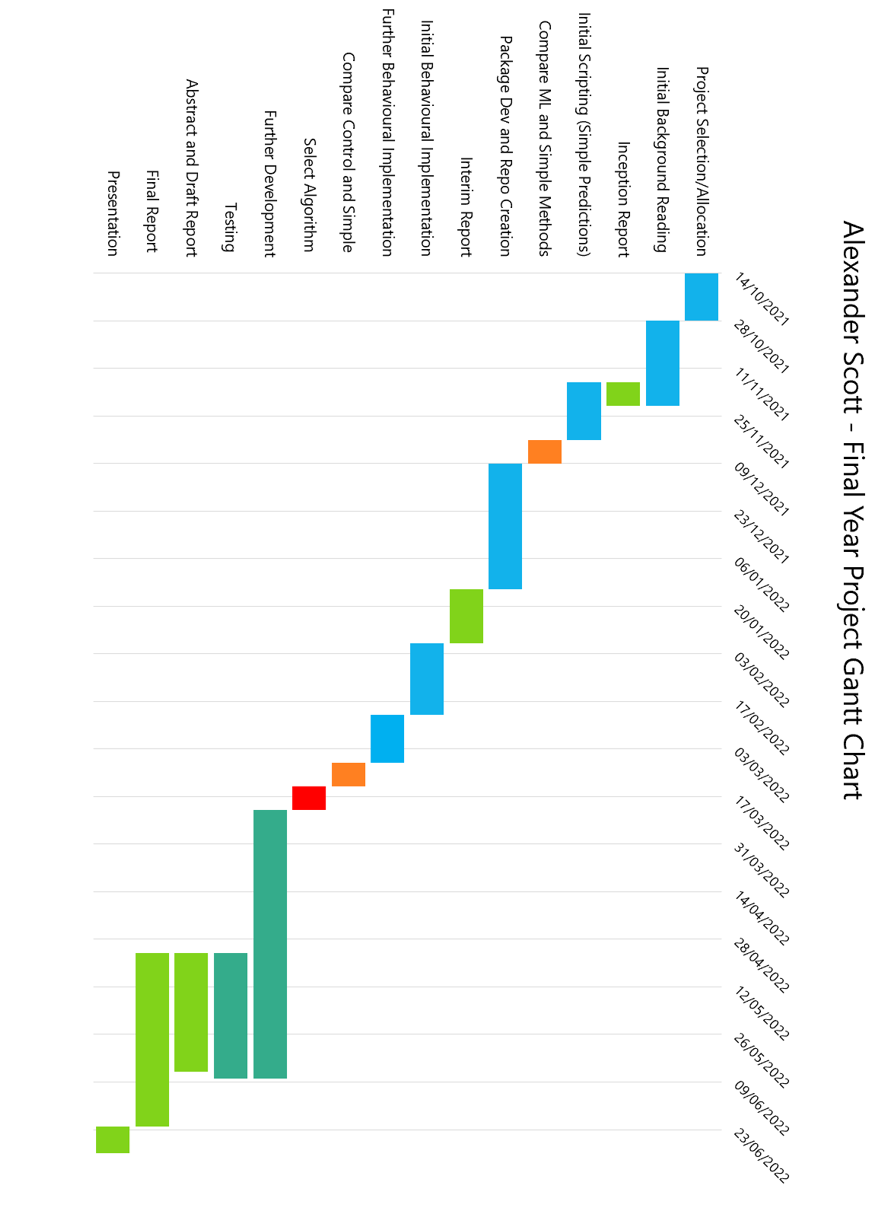
\includegraphics{Implementation/timescale.PNG}
    \caption{Gantt Chart showing Project Milestones}
    \label{fig:timescale}
\end{figure}

\section{Data Preparation}
\label{section: data_prep}

\noindent The methods of data preparation described below are essential to provide the package user with the ability to manipulate data as desired. Data Retrieval, Splitting, Standardisation and and Re-scaling form the basis of necessary data manipulation for processing by the implemented prediction algorithms. The full code Listing of the \textbf{Data.jl} which implements all the elements of data manipulation can be viewed in Listing \ref{lst: Data.jl}.

\subsection{Data Retrieval} 
\label{imp: data_ret}
The data sets that all prediction algorithms were tested on were retrieved from \textbf{Yahoo Finance}. Two main samples were used, \textbf{Apple} for the time period \textit{"2016-07-09"} to \textit {"2021-07-09"} and  \textbf{Amazon} for the time-period \textit{"2018-01-01"} to \textit{"2020-12-31"}.
The Apple sample had to be used in order to compare simple and machine learning methods as this was the sample used in last year's paper \cite{ml_paper}. Amazon was used to compare the simple and behavioural control implementation as it is an extremely stable stock and is less prone to rapid changes in price compared to those with lower market cap, it is considered by most investors to be very safe \cite{amazon}.  Additionally there were no other anomalies during this time period besides the COVID-19 pandemic. Therefore, this data set was chosen to test the prediction techniques as it was a fairly good representation of "normal" market behaviour. 

\noindent Although a specific time-period was selected for testing, the data retrieval methods were designed in such a way that the user of the package would have the flexibility to select any time-period and stock desired. Therefore, the user of the package would be able to perform all of the implemented prediction techniques to any stock they wish - shown in Listing \ref{lst: get_data}. 

\subsection{Splitting into Train and Test Data}
\noindent As with most algorithms, the data must be split into "training" and "testing" portions. Therefore, methods were implemented to allow the user to split-up the data accordingly. In the case of the testing done in this report, the data was split up into $\frac{2}{3}$ training data and $\frac{1}{3}$ testing data.

\subsection{Data Standardisation}

\noindent The retrieved data was then standardised according to the \textbf{mean} and \textbf{standard deviation} of the training data \cite{standard}. It is common to only standardise the data to have zero mean and unit standard deviation with regards to the \textit{training data} as this prevents information leakage between the training and test data \cite{why_standard}.

\begin{listing}
\caption{Description of Data Retrieval Function}
\label{lst: get_data}
\begin{minted}[mathescape,
              frame=lines,]{julia}

# get_data is used to import live_data from yahoo finance of a  
# selected stock tickr, in a specified range as well as, a  
# specified interval

function get_data(tickr::String, start::String, 
                  finish::String,range::String,    
                  int::String)
    live_data = yfinance.download(tickr, start, finish, period = 
                                  range, interval = int) 
    #import data from any period desired
    info = Pandas.DataFrame(live_data) # Wrap in a pandas DataFrame
    info = Pandas.reset_index(info) # set the index 
    info = DataFrames.DataFrame(info) # Convert to julia DataFrame
    Pandas.display(info) # display
    all_data = info
    all_data # return data
end

\end{minted}
\end{listing}

\subsection{Data Re-scaling}

\noindent Since the data was standardised before processing, methods needed to be implemented that enabled intuitive viewing of the price data after running the selected prediction algorithm. Thus, data re-scaling functions were added to the \textbf{Data.jl} file allowing the user to effectively compare the predictions generated to the true-valued test data.

\section{Simple Prediction Techniques}

After the necessary data prep described in Section \ref{section: data_prep}, the pre-processed sample was fed into a variety of simple prediction techniques. The most common and simple prediction techniques were implemented in order to establish a performance baseline. All techniques implemented are available for the package user to utilise as they see fit, these include:
\begin{itemize}
    \item Naive Prediction
    \item Simple Moving Average 
    \item Linear Predictors.
\end{itemize}

 \noindent All simple prediction methods are found and dedicated in the file \textbf{Simple.jl}, the full code listing can be viewed in Listing \ref{lst: Simple.jl}. The details of each prediction technique are described in further detail in the following sub-sections.
 
\subsection{Naive Prediction}

The Naive prediction is the simplest prediction algorithm that can be described as

\begin{equation}
    p_{i} = p_{i-n}
    \label{eqn: naive} 
\end{equation}

\noindent where, 

$i-n \geq 0$, $n \geq 1$, 

$p_i$ = predicted adjusted closing price on day $i$, 

$n$ = number of days prior to current day. 

\noindent In other words, the next-day prediction is equal to the the adjusted closing price of the stock $n$ days prior. In general, the selected value of $n$ is $n = 1$. 

\subsection{Simple Moving Average (SMA)}

The simple moving average prediction stems from Equation \ref{eqn: SMA} and is the second classical prediction algorithm implemented. It bases the following days prediction on the average of the previous specified time frame. For an array of price values, the average is taken within a moving window to make predictions. The prediction can be defined as, 


\begin{equation}
    \label{eqn: pred_sma}
    p_{i} = \frac{p_{i-n}+\dots+p_{i-1}}{n}
\end{equation}

\noindent where, 

$i-n \geq 0$, $n \geq 2$, 

$p_i$ = predicted adjusted closing price on day $i$, 

$n$ = number of days prior to current day. 

\subsection{Linear Prediction}
The third and final classical method of stock prediction used were linear predictors. It was similar to the moving average in the sense that the predictions were calculated within a moving window of user-specified size. The algorithm states that the next day’s price forecast lies on the line of best linear fit 
of the previous specified number of days. This line is calculated, and the y-value of the following day extracted. The implementation is best described as

\begin{equation}
    \label{eqn: pred_lin}
    p_{i} = An + b
\end{equation}

\noindent where, 

$i-n \geq 0$, $n \geq 2$, 

$p_i$ = predicted adjusted closing price on day $i$, 

$n$ = number of days used to calculate line of best fit,

$A$ = gradient of line of best fit for historical n days,

$b$ = y-intercept of line of best fit for historical n days. 

\noindent The code for the implementation is shown in Listing \ref{lst: lin_pred} as the implementation is slightly more complex compared to the Naive and SMA.

\begin{listing}[h]
\caption{Description of the Linear Prediction Function}
\label{lst: lin_pred}
\begin{minted}[mathescape,
              frame=lines,]{julia}

function linear_predict(data::Array)
    vector_data = vec(data)
    df = DataFrames.DataFrame(y = vector_data, x = 1:size(data,1))
    fm = @formula(y ~ x)
    model = lm(fm, df)
    slope = GLM.coef(model)[2]
    y_int = GLM.coef(model)[1]
    y = slope*(size(vector_data,1)) + y_int
    y
end

\end{minted}
\end{listing}

\section{Plotting}
The predictions generated by the aforementioned simple prediction techniques are then plotted.
Graphs and charts give the user a visual representation of their data as well as facilitate comparison and contrasting between different data sets. It is also a simple way of visualizing and double-checking expected results/predictions against training and test data. The file \textbf{Plotting.jl} contains all functions related to plotting that the package user would have access to - see \hyperlink{}{https://github.com/JuDO-dev/AirBorne.jl/blob/dev/src/Plotting.jl}. Shown in Figure \ref{fig:plot_example} is an example of a graph plotted after performing a simple moving average prediction $n = 3$, comparing predictions against the test data.

\begin{figure}
    \centering
    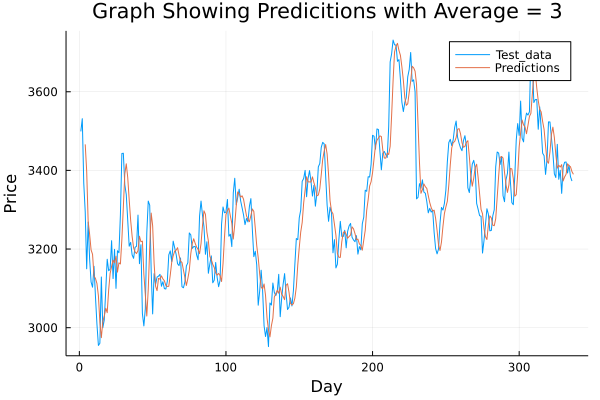
\includegraphics[width=1\columnwidth]{Implementation/Moving_Avgs_Test_data_3.png}
    \caption{Example of SMA Plot Comparing Predictions to Test Data}
    \label{fig:plot_example}
\end{figure}

\section{Errors}
In addition to plotting, the predictions generated need to be compared numerically, \textbf{Errors.jl} contains all relevant methods of error calculation available to the package user. The implementation can be viewed by accessing  \hyperlink{label}{https://github.com/JuDO-dev/AirBorne.jl/blob/dev/src/Errors.jl}
. The intended use of the plots generated as well as the errors are further explored in Chapter \ref{chapter: Testing} as well as the results in Chapter \ref{chapter: Results}.

\section{Behavioural Control Theory Implementation}

\subsection{Prediction Algorithm}
The implementation of the behavioural control theory explored in Section \ref{back: behavioural} is a several step process that can be summarized in the following steps:
\begin{enumerate}
    \item Select a data sample
    \item Prepare data for processing
    \item Construct Hankel Matrix
    \item Form \& Solve Data Estimation Problem
    \item Extract Predictions 
\end{enumerate}
    
\noindent The details of the steps above will be explored in the following sub-sections to ensure the reader's full understanding of the process. A visual overview of the functions involved and their relationships with the steps described can be viewed in Figure \ref{fig: package_flow}.

\subsubsection{Data Sample Selection}

As stated in Section \ref{imp: data_ret} the selected data sample that the algorithm was tested on was the stock, \textbf{Amazon} over the period  \textit{"2018-01-01"} to \textit{"2021-12-31"}. The reasoning for this sample selection can also be found in \ref{imp: data_ret}.

\subsubsection{Data Preparation}
Utilizing the functions defined in the \textbf{Data.jl} file, the data was split up into train and test data and standardised such that the data had zero mean and unit standard deviation. Shown in Listing \ref{lst: Data.jl} are the functions used.

\subsubsection{Hankel Matrix Construction}
The Hankel matrix of user-specified depth $L$, is then constructed using the training data- see Listing \ref{lst: hank}. The definition of a Hankel matrix is stated in Section \ref{back: behavioural} Equation \ref{eqn: hank}. The implementation of the Hankel matrix construction was written such that the matrix can be formed from multiple vectors for users that desire to run the algorithm on a combination of different inputs e.g. price and volume data simultaneously. To view the implementation see Listing \ref{lst: hank}.

\subsubsection{Optimisation}

Utilizing the Hankel matrix putting the data into relevant form, the L1-norm optimisation problem stated in Section \ref{back: behavioural} Equation \ref{eqn: opt} is solved using Lasso Regression utilizing the \textbf{Convex.jl} package and the predictions are retrieved. The function used to perform the regression is shown in Listing \ref{lst: lasso}. After the optimisation problem is solved relevant plots and errors are generated and comparisons made between those generated by the simple prediction techniques. 

\section{Buy/Sell Implementation}
\label{section: buy_sell}

\subsection{Errors and Statistics}

In order to implement the Buy/Sell Algorithm, the test data is split into two parts, an overview is given in Figure \ref{fig: Buy_sell}. The first set of test data is used to calculate errors and statistical data associated with the stock to produce confidence intervals. This is done by calculating the relative error between the predictions and \textit{test data 1} then plotting a histogram. The package \textbf{Distributions.jl} is used to fit a normal distribution to the error data. The user is then able to specify a desired confidence interval, e.g. $90\%$ and two values that bound $90\%$ of the area underneath the distribution are returned by making use of the \textit{quantile} function provided by the package. The confidence interval is used to to determine when to buy or sell the stock when testing on \textit{test data 2}. The implementation can be found in the files \textbf{Errors.jl} and \textbf{Buy\_sell.jl} by accessing \hyperlink{label}{https://github.com/JuDO-dev/AirBorne.jl/blob/dev/src}. Furthermore, the green line shown is the result of performing a kernel density estimation on the histogram data, it is an attempt to estimate the probability density function instead of fitting it to a normal. In this case, fitting the distribution to a normal is used for simplicity. In future, exploring the use of kernel density estimation to obtain the confidence interval values may improve the statistical analysis.
Figure \ref{fig: hist_example} illustrates an example of the statistical analysis performed on the first half of the test data.

\subsection{Strategy}
\label{subsection: buy_sell_strat}

The strategy implemented when buying and selling the shares of the stock over the second half of the test data (\textbf{126 days}), for a prediction one or more days ahead was based on the upper and lower bounds calculated from the first half of the test data. The decision made on day $i$ was made as follows:

\begin{equation}\label{eqn: buy_sell}
    D_{i} =
    \begin{cases}
        B_{i}, &  p_{i} \geq c_{i}.bound_{upper} \\
        S_{i}, &  p_{i} \leq c_{i}.bound_{lower} \\
        H_{i}, &  c_{i}.bound_{upper} > p_{i} > c_{i}.bound_{lower} \\
    \end{cases}
\end{equation}

\noindent where, 

$D_{i}$ = Decision on day $i$, 

$B_{i}$ = Buy decision on day $i$, 

$S_{i}$ = Sell decision on day $i$, 

$H_{i}$ = Hold decision on day $i$, 

$p_{i}$ = Prediction on day $i$ one or more days ahead, 

$c_i$ = Current price on day $i$, 

$bound_{upper}$ = upper bound, 

$bound_{lower}$ = lower bound. 

\noindent It is important to note that in reality, the process of buying and selling shares is significantly more complex as investors are interested in many other factors that affect the decision to buy/sell or hold. Factors not taken into account for simplicity include, 

\begin{itemize}
    \item Different Buy/Sell signals 
    
    The prices used in the strategy are the adjusted closing price of the stock at the end of the day. In reality, stocks are not traded at a single price, there are usually two prices associated with buying and selling a security. There is an ask price and a bid price. The asking price of a stock is defined as the lowest possible price that a a shareholder is willing to sell their shares for \cite{bid_ask}. The bid price is the highest price a buyer is willing to pay for the security \cite{bid_ask}. The difference between these price is called the spread \cite{bid_ask}. Stock are not bought and sold at the adjusted closing price but rather the the bid and ask price this often fluctuates throughout the day and thus, can have an effect on profits depending on the time of day the the stock is bought/sold.
    
    \item The period associated with a Buy/Sell order 
    
    When an order to buy/sell a stock is placed, the investor can specify how long they would like the offer to stand. If their offer is not accepted over the specified period, it will be withdrawn likely because it may either be too low or too high compared to the current bid or ask price. The implementation assumes that orders are filled immediately at the current price, when in reality the current price is the price of the last trade whether a buy or sell \cite{bid_ask}.   
    
    \item Order Type
    
    When an investor issues an order to buy or sell stock at a specified price it is not guaranteed that the transaction will occur at that exact price, it may differ slightly. The actual price at which the transaction occurs is dependant on the order type. Two types of orders include there are market orders and limit orders which have different specifications. A market order will generally be filled near to the bid price if buying or near to the ask price if selling \cite{orders}. A limit order will be filled at a specific price or lower for a buy limit order and at a specific price or higher for a sell limit order \cite{orders}. The current implementation assumes that all orders at filled at the current market price.
\end{itemize}

\begin{figure}[h]
    \centering
    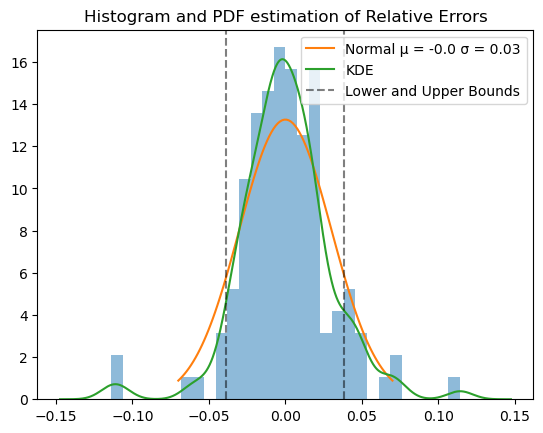
\includegraphics[width=1\columnwidth]{Implementation/hist_example.png}
    \caption{Example of Histogram, estimated PDF and Bounds}
    \label{fig: hist_example}
\end{figure}











 







